\documentclass[10pt]{article}
\usepackage[margin=0.75in]{geometry}
\usepackage{graphicx,hyperref,longtable}
\begin{document}
\section*{CMPE 249 Track A: controlled detector evaluation}
Abstract. This study compares pretrained YOLOv8n, YOLO11n and RT-DETR-L on full COCO val2017 and a fixed 500-image sample of prepared KITTI validation data. All primary comparisons use a single CUDA device, input size 512, batch one and FP32. Results come from saved original-coordinate predictions evaluated with official pycocotools COCOeval. A three-class evaluation supports domain comparison, while bicycle/cyclist is reported separately. Efficiency is measured on decoded images with synchronization, warmup, repeated measurements and fresh model processes. No model was trained or fine-tuned.


Question and scope. How do these three supplied checkpoints trade accuracy for prediction latency, and how do measured shared-class scores change between COCO scenes and the driving domain? The models cover two detector families. Their capacities differ substantially, so the experiment compares deployable checkpoint configurations rather than isolating architecture effects. Published benchmark claims are context, not substitutes for local measurements [1-6].


Execution evidence. The local environment is NVIDIA GeForce RTX 5070 Ti Laptop GPU, PyTorch 2.14.1+cu130, Ultralytics 8.4.198 and Python 3.13.6. Audit: 5000 COCO images, 36781 annotations, 500 KITTI images sampled from 1496. The timing set contains exactly 19 supported images. All 15 assertion-based evaluator checks passed; all three detectors produced CUDA results with hooks verifying shape, dtype and evaluation state.


Reading the results. AP values are fractions on [0,1]; differences described in percentage points multiply AP differences by 100. COCO all-class AP and the shared-class transfer metric answer different questions and are never subtracted. Converted KITTI scores use COCO rules and are not official KITTI benchmark scores. Detailed commands, hashes, predictions, evaluator arrays and error history accompany this report.


\begin{longtable}{llll}
Model & COCO AP & AP50 & AP75 \\
yolov8n.pt & 0.352 & 0.496 & 0.381 \\
yolo11n.pt & 0.364 & 0.511 & 0.392 \\
rtdetr-l.pt & 0.508 & 0.693 & 0.546 \\
\end{longtable}
\newpage
\section*{2. Models and inspected implementation}
YOLOv8n and YOLO11n use multi-scale convolutional detection. The installed YOLOv8 configuration contains C2f feature blocks and SPPF, with top-down and bottom-up feature fusion feeding a Detect head at P3/P4/P5. YOLO11 uses C3k2 blocks and C2PSA while retaining multi-scale detection. Both selected checkpoints pass through DetectionPredictor.postprocess, class-aware non-maximum suppression and original-image coordinate restoration [5,6,8].


The supplied RT-DETR-L configuration has an HGStem/HGBlock backbone, AIFI within-scale interaction, cross-scale RepC3 fusion and an RTDETRDecoder. Its set-prediction lineage uses bipartite assignment, as in DETR [2,3]. This installed RTDETRPredictor has scale\_fill=True and converts normalized center/size predictions to original-image corners. It filters confidence and caps predictions without NMS. The supplied checkpoint should not be described as a ResNet variant merely because another RT-DETR implementation uses that backbone [9].


Loss and assignment context. Inspected local code contains TaskAlignedAssigner, BCEWithLogits classification and BboxLoss with distributional box regression for the YOLO path. The RT-DETR loss contains Hungarian matching and class, box/GIoU, auxiliary and denoising terms. These explain training design; no training loss was measured in this project. Inference capacity is reported below from actual loaded parameters before fusion.


Implementation evidence. architecture\_notes.md and implementation\_snapshot/index.json identify copied installed source files and SHA-256 hashes. experiments/*/model\_evidence.json records module counts, parameter dtypes, selected predictor and actual processed tensors. Official documentation describes current behavior but may evolve; the installed snapshot grounds version-specific statements. Equal nominal input sizes still give different image transformations, so preprocessing is part of the checkpoint comparison.


\begin{longtable}{llll}
Model & Parameters & Predictor & Resize \\
yolov8n.pt & 3157200 & DetectionPredictor & letterbox \\
yolo11n.pt & 2624080 & DetectionPredictor & letterbox \\
rtdetr-l.pt & 32970476 & RTDETRPredictor & stretch \\
\end{longtable}
\newpage
\section*{3. Data, taxonomy and validation}
COCO val2017 uses all 5,000 official image IDs and 80 annotated categories [1]. Predictions map class names to the actual sparse category IDs in instances\_val2017.json. The original COCO areas and crowd flags are preserved. KITTI uses the existing prepared Ultralytics images/val split, not the official test server [4]. A sorted parent list is sampled once with Python random.Random(42).sample; the exact 500 selected paths and hashes are saved. A separately seeded 200-image sample of those 500 supplies labeled ablations.


Primary taxonomy: person maps to pedestrian, car to car, truck to truck. KITTI separates vans from cars and sitting persons from pedestrians; those labels are excluded from scored GT. Bicycle to cyclist is an approximate supplementary mapping because the rider and box extents need not match a bicycle-only annotation. No numeric class ID is assumed interchangeable. Nonmapped predictions do not enter the shared-class score.


Prepared YOLO annotations lack DontCare, truncation, occlusion and difficulty. No difficulty filtering or ignore-region suppression is possible. Excluded classes are not scored as GT; mapped predictions over those objects can count as false positives. Other predicted classes are excluded only for shared-class evaluation. These are COCO-style mapped scores, not official KITTI scores.


Annotation validation checks ID uniqueness, category references, dimensions, finite coordinates, positive boxes and image decodability. Prepared KITTI normalized center/size labels are restored to original pixels and clipped at image bounds. Missing label files raise errors; empty files are recorded as legitimate negatives. This selected subset has no missing or empty label files. Source labels remain unchanged. Several original-resolution GT overlays are saved for visual checks.


Size interpretation. COCO retains original area metadata, usually segmentation-derived. Converted KITTI area is clipped bounding-box width times height. COCOeval size strata are therefore reproducible within each dataset but are not physically equivalent across datasets. Domain effects cannot be reduced to an architecture ranking.


\begin{longtable}{llll}
Concept & COCO GT & KITTI GT & Role \\
person & 11004 & 296 & primary \\
car & 1932 & 1860 & primary \\
truck & 415 & 79 & primary \\
bicycle & 316 & 114 & approximate \\
\end{longtable}
\begin{center}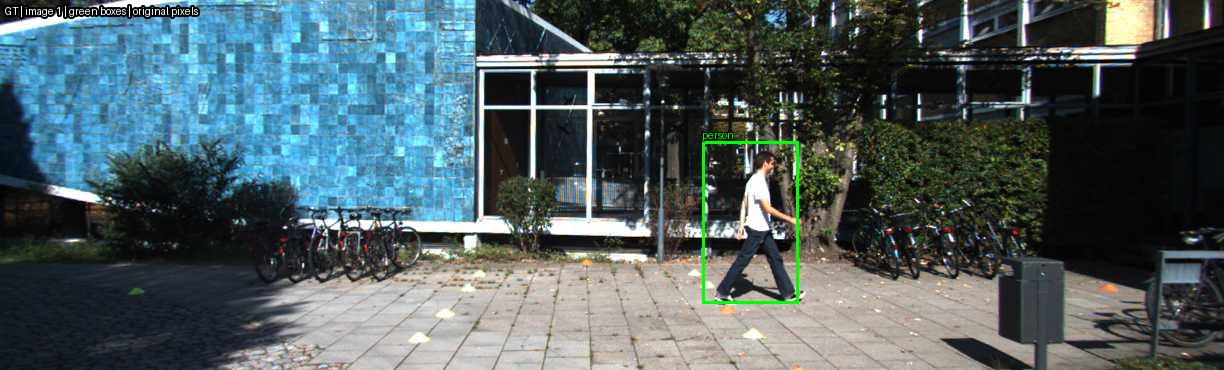
\includegraphics[width=0.92\linewidth,height=0.42\textheight,keepaspectratio]{figures/1.jpg}\end{center}
\newpage
\section*{4. Evaluation protocol and primary accuracy}
Primary settings: 512 input, batch 1, FP32, device 0, confidence .001, export cap 300. YOLO NMS IoU is .70. RT-DETR is NMS-free. rect=False forces square processed inputs; YOLO uses aspect-preserving resize/padding while RT-DETR stretches. BGR pixels become RGB floats divided by 255. Hooks assert CUDA, the requested float dtype, batch one, no gradients and evaluation mode. Framework classes are selected explicitly for each detector.


Official COCOeval bbox evaluation uses IoU thresholds .50:.05:.95, recall sampling at 101 points and maxDets [1,10,100] [7]. Saved exports precede metrics, so evaluation can run without another GPU pass. Arrays preserve precision, recall, scores, categories, image IDs and thresholds. AP50-95, AP50, AP75, size AP, AR1/10/100 and per-class AP/GT counts appear in CSV/LaTeX tables. Undefined values are null/N/A rather than zero.


Evaluator tests cover perfect and empty predictions, duplicates, wrong class, wrong localization, absent GT classes, overlapping GT requiring an unmatched alternative, coordinate conversion/clipping, reversed/nonfinite boxes, missing versus empty labels, unknown categories and invalid/duplicate image IDs. The alternative-match case confirms two true positives at IoU .50. Duplicate predictions after complete recall can leave interpolated AP at one; that expected behavior is asserted, not treated as a failure.


The primary accuracy chart uses only person, car and truck on both datasets. Its macro average is calculated over the same categories with the same evaluator. The separate all-80 COCO result measures breadth. The KITTI all-vocabulary export also contains supplementary bicycle/cyclist, which is not the primary shared transfer macro.


\begin{longtable}{lllll}
Model & COCO APs & APm & APl & AR100 \\
yolov8n.pt & 0.147 & 0.384 & 0.546 & 0.521 \\
yolo11n.pt & 0.153 & 0.397 & 0.565 & 0.527 \\
rtdetr-l.pt & 0.312 & 0.555 & 0.708 & 0.696 \\
\end{longtable}
\begin{center}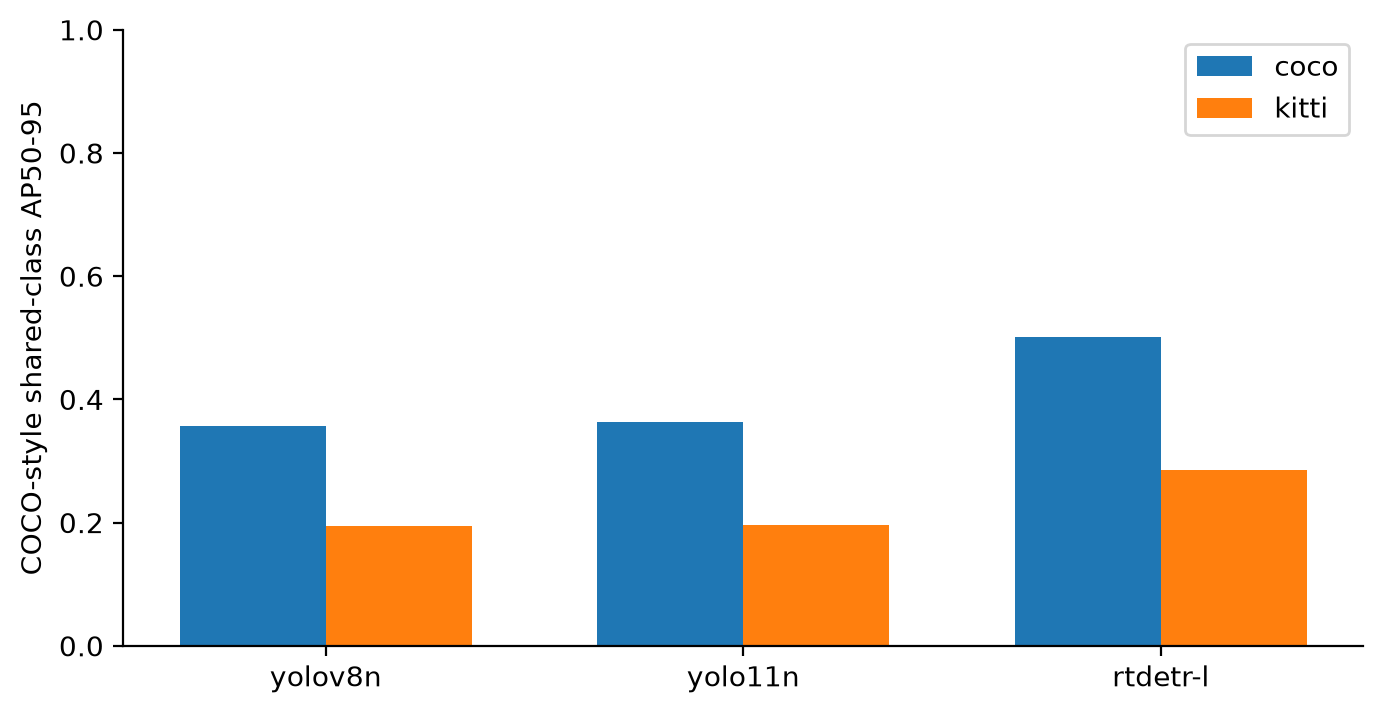
\includegraphics[width=0.92\linewidth,height=0.42\textheight,keepaspectratio]{figures/shared_accuracy.png}\end{center}
\newpage
\section*{5. Analysis I: cross-dataset behavior}
yolov8n.pt: shared AP changes from 0.3567 to 0.1943, a descriptive difference of -16.24 percentage points. Supplementary KITTI bicycle/cyclist AP is 0.0037. The per-class table and paired plot show whether the macro hides contrasting class behavior.


yolo11n.pt: shared AP changes from 0.3632 to 0.1969, a descriptive difference of -16.63 percentage points. Supplementary KITTI bicycle/cyclist AP is 0.0017. The per-class table and paired plot show whether the macro hides contrasting class behavior.


rtdetr-l.pt: shared AP changes from 0.5017 to 0.2860, a descriptive difference of -21.57 percentage points. Supplementary KITTI bicycle/cyclist AP is 0.0011. The per-class table and paired plot show whether the macro hides contrasting class behavior.


The macro drop does not apply uniformly across classes. Car AP changes are yolov8n: +4.54 points, yolo11n: +3.40 points, rtdetr-l: +1.55 points. The paired plot shows person and truck reductions alongside these car increases. Class composition and taxonomy therefore matter to interpretation.


These are zero-shot observations from COCO-pretrained models. A change in score can reflect image composition, object frequency, camera viewpoint, object scale, annotation conventions or predictor preprocessing. It does not isolate generalization as a causal property of one architecture. KITTI has many cars but fewer trucks and pedestrians, yet AP is macro averaged by class; the count imbalance changes uncertainty and examples available rather than assigning a car-weighted AP.


The bicycle/cyclist comparison must remain visible even when poor. A cyclist annotation can cover both rider and vehicle, whereas COCO can separately annotate person and bicycle. Car/van and pedestrian/sitting-person distinctions also produce apparent errors under the selected mapping. Missing DontCare masks can penalize detections an official KITTI protocol might ignore. Preserve these caveats when presenting the numerical transfer differences.


\begin{center}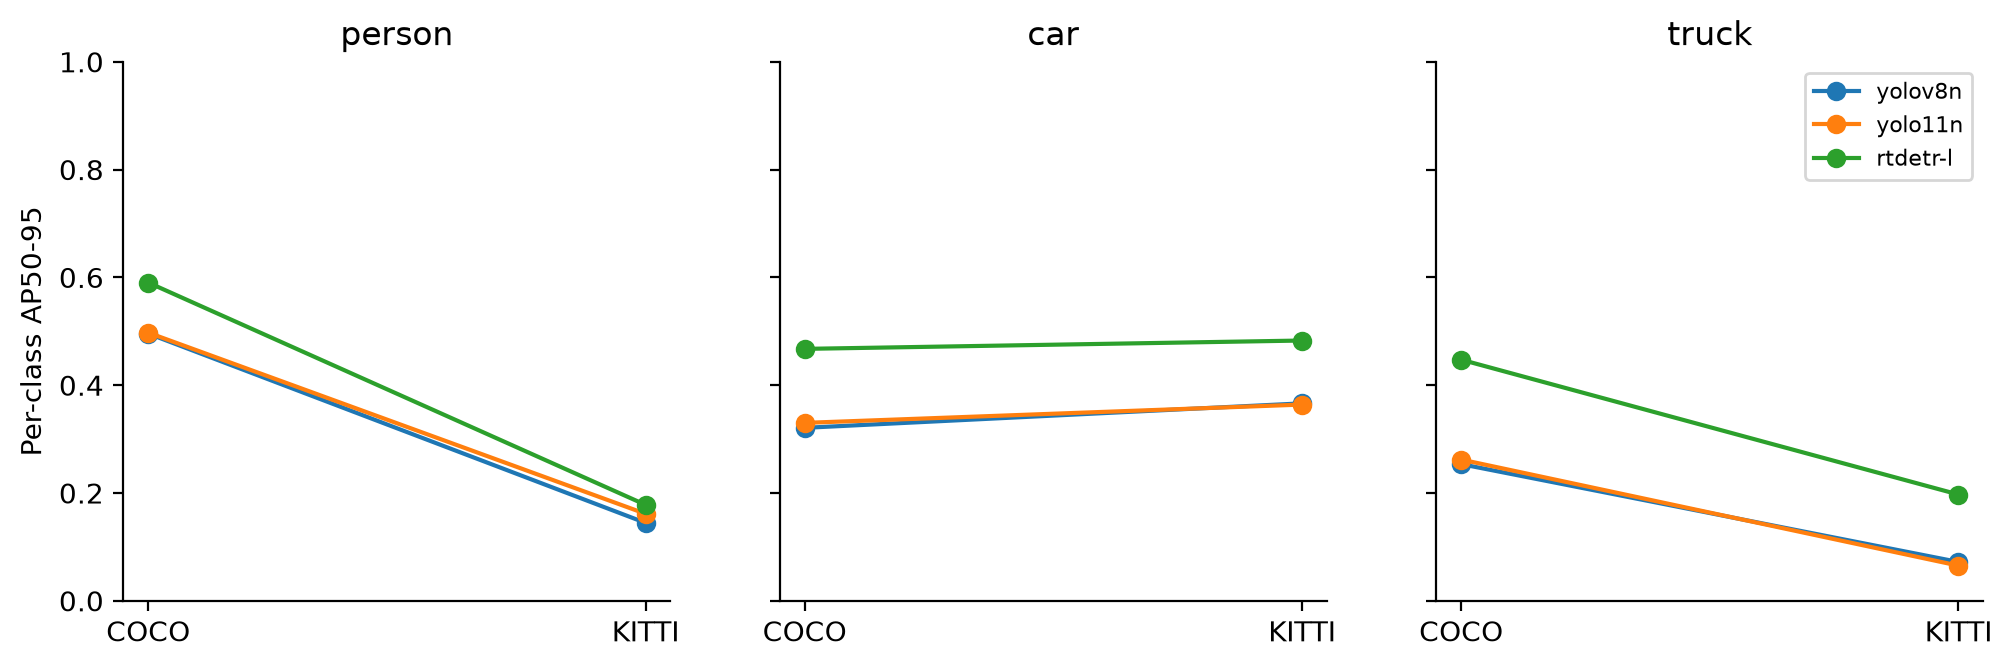
\includegraphics[width=0.92\linewidth,height=0.42\textheight,keepaspectratio]{figures/per_class_transfer.png}\end{center}
\newpage
\section*{6. Analysis II: latency, memory and parameter changes}
Timing uses a separate .25 confidence baseline. All 19 decoded images are preloaded outside timing. Each fresh subprocess loads one model, runs 10 warmup calls and five timed repetitions per image. A monotonic CPU clock and CUDA synchronization surround each full model.predict call. This includes resize, H2D, normalization, inference, postprocessing, coordinate restoration and API overhead; it excludes disk read/decode, CPU export and drawing. Framework inference timing isolates the forward pass. The sample count is 95 timed calls per configuration.


FPS is 1000 divided by mean per-image full-prediction latency. Tables retain median, p95, standard deviation, repetition means and between-repetition spread. Peak allocated and reserved memory come from the PyTorch allocator after warmup; they are not total device VRAM. The manifest captures power scheme, battery status and nvidia-smi when available. Laptop temperature, clocks and concurrent activity can vary; small differences relative to observed spread do not establish a stable winner.


One-factor changes around the timing baseline cover 384/512/640 resolution, verified FP16 versus FP32, confidence .10/.25/.50, and YOLO-only NMS IoU .50/.70. Identical settings are deduplicated; RT-DETR has no NMS sweep. Labeled ablations use a fixed 200-image KITTI sample at .001 confidence for distinct resolution/precision settings. The corresponding 512 FP32 predictions are reused from the primary run. Unlabeled output counts describe filtering, not measured recall. The observed YOLO latency curves are not monotonic with resolution; clock/host variability and overhead are plausible explanations, not experimentally isolated causes.


\begin{longtable}{lllll}
Model & Full ms & Forward ms & FPS & Alloc MiB \\
yolov8n.pt & 10.587 & 7.777 & 94.451 & 40.406 \\
yolo11n.pt & 14.104 & 10.979 & 70.900 & 68.243 \\
rtdetr-l.pt & 27.270 & 24.609 & 36.670 & 237.213 \\
\end{longtable}
\begin{center}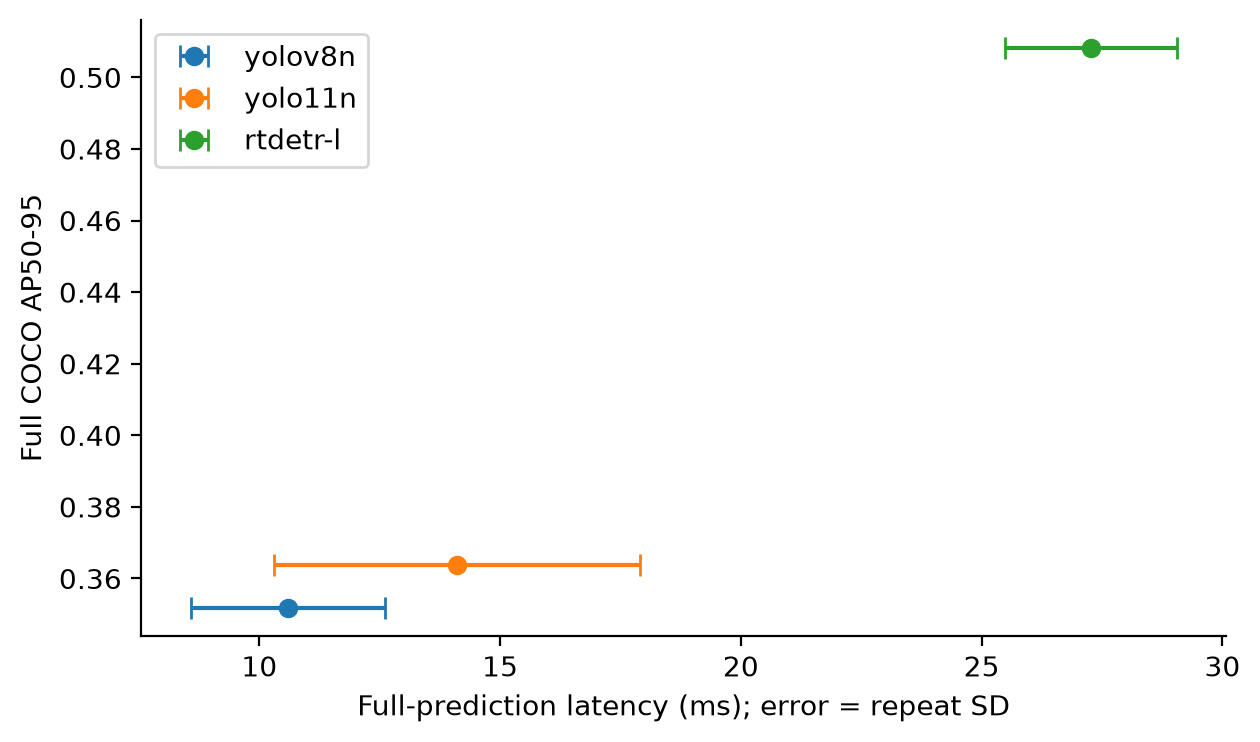
\includegraphics[width=0.92\linewidth,height=0.42\textheight,keepaspectratio]{figures/speed_accuracy.png}\end{center}
\begin{center}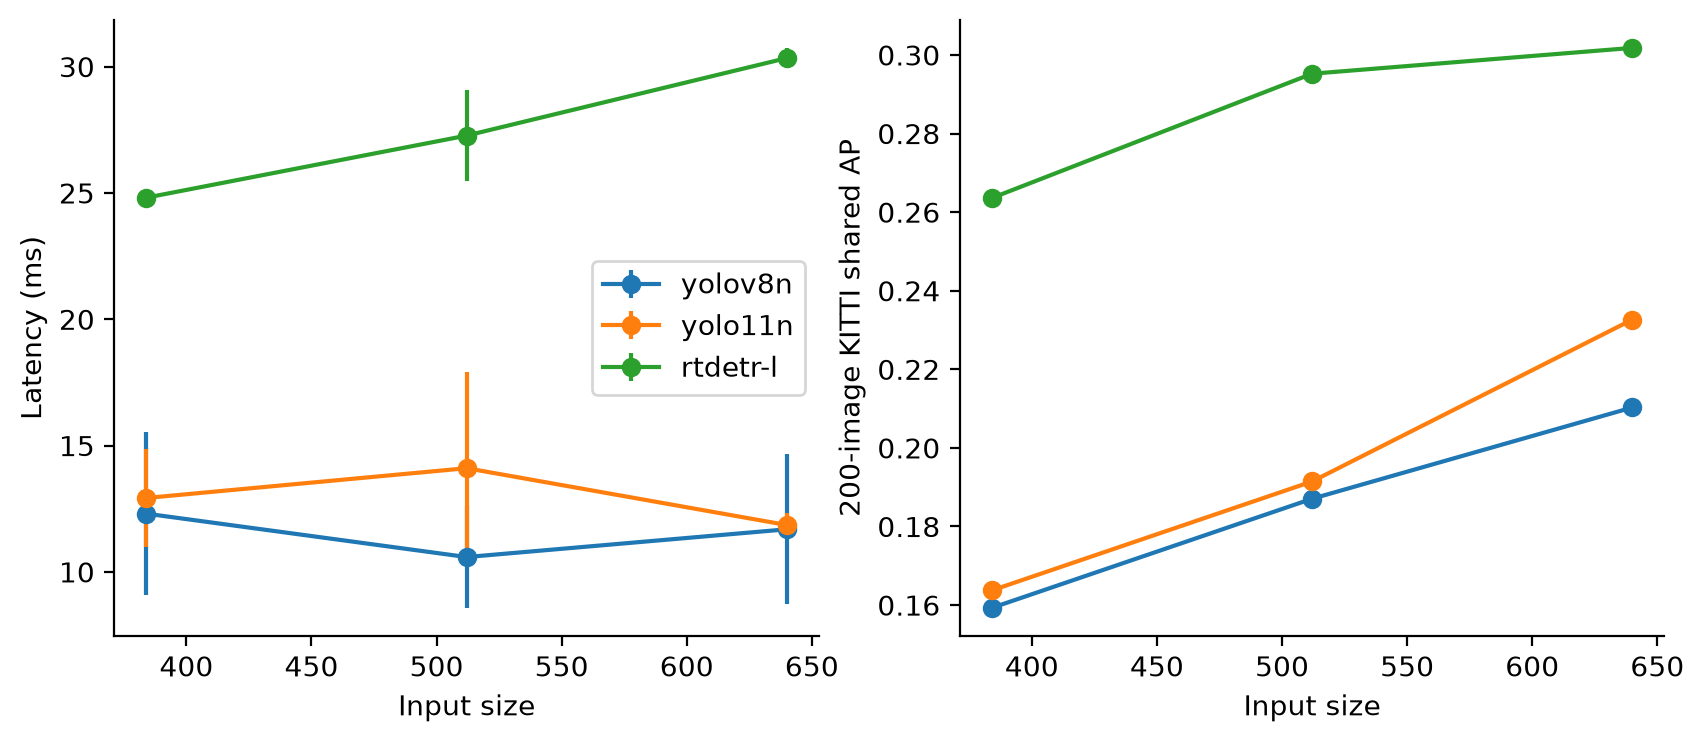
\includegraphics[width=0.92\linewidth,height=0.42\textheight,keepaspectratio]{figures/parameter_sensitivity.png}\end{center}
\newpage
\section*{7. Qualitative failures and limitations}
Six different annotated KITTI scenes are selected with recorded rules: most small GT objects, most mapped objects, most pedestrians, most trucks, maximum overlap fraction between GT boxes, and the highest shared-class false-positive count for YOLOv8n at IoU .50/confidence .25. Exact selection IDs and reasons are saved. Green denotes GT and blue denotes model predictions at the same visualization threshold. Full panels include all three models; separate crops preserve readable object detail. Captions report image IDs and settings. Overlap does not automatically prove physical occlusion; the prepared labels omit occlusion attributes.


The crop below comes from the selected false-positive scene; the corresponding original-resolution full panel is included in figures/. Its selection uses official COCOeval assignments, not a visual guess. Per-image TP/FP/FN diagnostics are saved for the primary shared classes at IoU .50 and confidence .25. An unmatched prediction can reflect wrong class/localization, excluded taxonomy, duplicate output or missing ignore metadata; the panel alone does not prove its cause. Similarly, a small or occluded object is a plausible source of difficulty, not evidence for an unmeasured mechanism.


Limits and conclusions. The results support checkpoint-level speed/accuracy choices under the measured protocol and descriptive domain comparisons. They do not establish performance on another device, precision backend or application distribution. The validation sample is fixed, not an independent official KITTI benchmark. No training, threshold selection or expensive extra model family was added. Reported uncertainty concerns timing repetition, not confidence bounds for AP. Complete raw exports remain available for additional diagnostics.


\begin{center}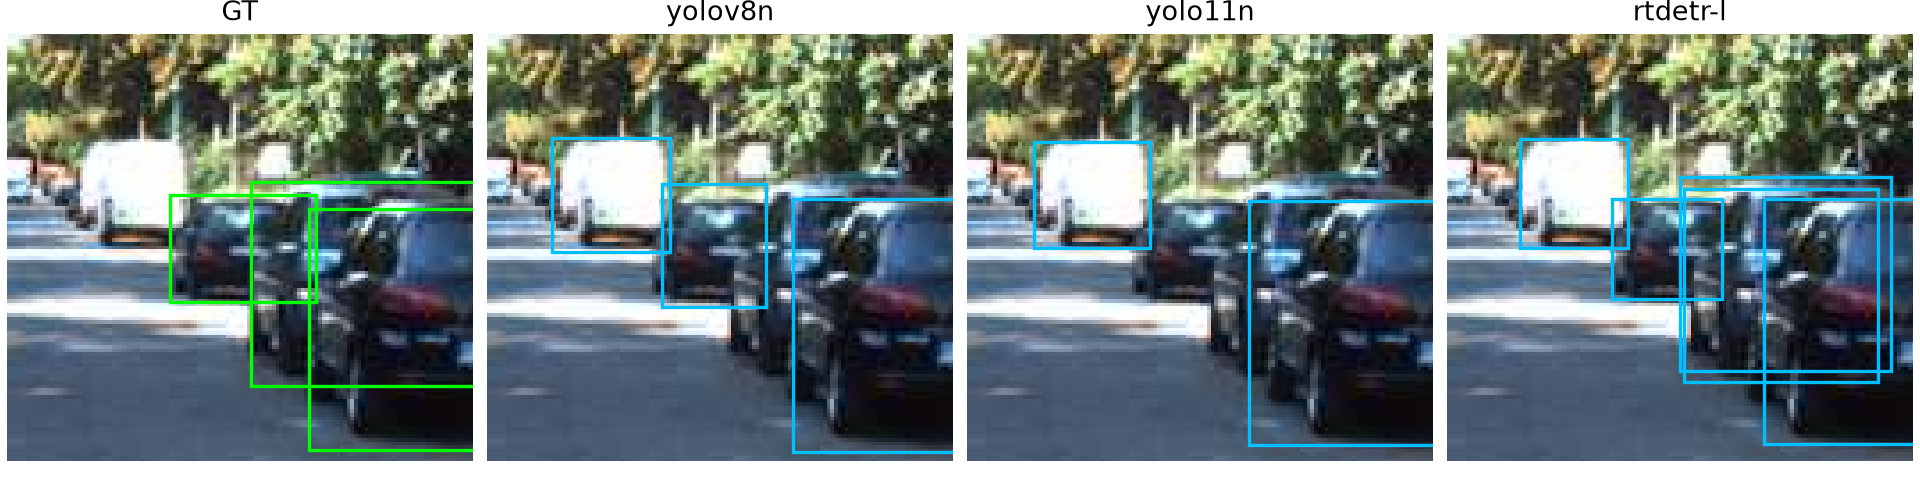
\includegraphics[width=0.92\linewidth,height=0.42\textheight,keepaspectratio]{figures/crop_420.png}\end{center}
\newpage
\section*{8. Reproducibility, references and AI-use statement}
Persistent run: results\_verified/20261103\_track\_a. Resume from the project root: dtect/Scripts/python.exe run\_track\_a.py --stage all --run-id 20261103\_track\_a --resume. Config, exact commands, append-only events, dataset manifests, checkpoint hashes and locked dependencies are included. Individual stages support independent reproduction. A saved KITTI prediction export was evaluated again and every shared metric reconciled exactly without GPU inference.


The run retains encountered implementation errors and recovery events; successful checks do not erase earlier failures. Compatible jobs reuse code/config/input/checkpoint signatures. Original project results were not promoted into this run. Archives omit datasets, checkpoints and environments; the separate prediction/evidence archive contains raw exports and GT needed for metric reproduction.


AI-use statement. An AI coding agent implemented the workflow, executed local checks and experiments, inspected source files, consulted the author/official reference pages and generated analysis/report assets from saved outputs. Automated assertions and visual inspection provide the verification described here. The student has not been represented as independently checking the code, results, references or prose; review and understanding before submission remain the student’s responsibility.


References (author/official pages checked 2026-11-03):


[1] Lin et al. Microsoft COCO: Common Objects in Context. ECCV 2014. https://arxiv.org/abs/1405.0312


[2] Carion et al. End-to-End Object Detection with Transformers. ECCV 2020. https://arxiv.org/abs/2005.12872


[3] Zhao et al. DETRs Beat YOLOs on Real-time Object Detection. CVPR 2024. https://arxiv.org/abs/2304.08069


[4] Geiger, Lenz and Urtasun. Are we ready for Autonomous Driving? The KITTI Vision Benchmark Suite. CVPR 2012. https://www.cvlibs.net/publications/Geiger2012CVPR.pdf


[5] Ultralytics. YOLOv8 model documentation. https://docs.ultralytics.com/models/yolov8/


[6] Ultralytics. YOLO11 model documentation. https://docs.ultralytics.com/models/yolo11/


[7] COCO Consortium. Official Python COCOeval implementation. https://github.com/cocodataset/cocoapi/blob/master/PythonAPI/pycocotools/cocoeval.py


[8] Ultralytics. Official framework source repository. https://github.com/ultralytics/ultralytics


[9] Ultralytics. RT-DETR model documentation. https://docs.ultralytics.com/models/rtdetr/


\end{document}